
\documentclass[a4paper,11pt]{article}
\usepackage[a4paper, margin=8em]{geometry}

% usa i pacchetti per la scrittura in italiano
\usepackage[french,italian]{babel}
\usepackage[T1]{fontenc}
\usepackage[utf8]{inputenc}
\frenchspacing 

% usa i pacchetti per la formattazione matematica
\usepackage{amsmath, amssymb, amsthm, amsfonts}

% usa altri pacchetti
\usepackage{gensymb}
\usepackage{hyperref}
\usepackage{standalone}

\usepackage{colortbl}

\usepackage{xstring}
\usepackage{karnaugh-map}

% imposta il titolo
\title{Computer Architectures notes}
\author{Luca Seggiani}
\date{2026}

% imposta lo stile
% usa helvetica
\usepackage[scaled]{helvet}
% usa palatino
\usepackage{palatino}
% usa un font monospazio guardabile
\usepackage{lmodern}

\renewcommand{\rmdefault}{ppl}
\renewcommand{\sfdefault}{phv}
\renewcommand{\ttdefault}{lmtt}

% circuiti
\usepackage{circuitikz}
\usetikzlibrary{babel}

% testo cerchiato
\newcommand*\circled[1]{\tikz[baseline=(char.base)]{
            \node[shape=circle,draw,inner sep=2pt] (char) {#1};}}

% disponi il titolo
\makeatletter
\renewcommand{\maketitle} {
	\begin{center} 
		\begin{minipage}[t]{.8\textwidth}
			\textsf{\huge\bfseries \@title} 
		\end{minipage}%
		\begin{minipage}[t]{.2\textwidth}
			\raggedleft \vspace{-1.65em}
			\textsf{\small \@author} \vfill
			\textsf{\small \@date}
		\end{minipage}
		\par
	\end{center}

	\thispagestyle{empty}
	\pagestyle{fancy}
}
\makeatother

% disponi teoremi
\usepackage{tcolorbox}
\newtcolorbox[auto counter, number within=section]{theorem}[2][]{%
	colback=blue!10, 
	colframe=blue!40!black, 
	sharp corners=northwest,
	fonttitle=\sffamily\bfseries, 
	title=Theorem~\thetcbcounter: #2, 
	#1
}

% disponi definizioni
\newtcolorbox[auto counter, number within=section]{definition}[2][]{%
	colback=red!10,
	colframe=red!40!black,
	sharp corners=northwest,
	fonttitle=\sffamily\bfseries,
	title=Definition~\thetcbcounter: #2,
	#1
}

% disponi codice
\usepackage{listings}
\usepackage[table]{xcolor}

\definecolor{codegreen}{rgb}{0,0.6,0}
\definecolor{codegray}{rgb}{0.5,0.5,0.5}
\definecolor{codepurple}{rgb}{0.58,0,0.82}
\definecolor{backcolour}{rgb}{0.95,0.95,0.92}

\lstdefinestyle{codestyle}{
		backgroundcolor=\color{black!5}, 
		commentstyle=\color{codegreen},
		keywordstyle=\bfseries\color{magenta},
		numberstyle=\sffamily\tiny\color{black!60},
		stringstyle=\color{green!50!black},
		basicstyle=\ttfamily\footnotesize,
		breakatwhitespace=false,         
		breaklines=true,                 
		captionpos=b,                    
		keepspaces=true,                 
		numbers=left,                    
		numbersep=5pt,                  
		showspaces=false,                
		showstringspaces=false,
		showtabs=false,                  
		tabsize=2
}

\lstdefinestyle{shellstyle}{
		backgroundcolor=\color{black!5}, 
		basicstyle=\ttfamily\footnotesize\color{black}, 
		commentstyle=\color{black}, 
		keywordstyle=\color{black},
		numberstyle=\color{black!5},
		stringstyle=\color{black}, 
		showspaces=false,
		showstringspaces=false, 
		showtabs=false, 
		tabsize=2, 
		numbers=none, 
		breaklines=true
}

\lstdefinelanguage{x86}{ 
  keywords={AAA, AAD, AAM, AAS, ADC, ADCB, ADCW, ADCL, ADD, ADDB, ADDW, ADDL, AND, ANDB, ANDW, ANDL,
        ARPL, BOUND, BSF, BSFL, BSFW, BSR, BSRL, BSRW, BSWAP, BT, BTC, BTCB, BTCW, BTCL, BTR, 
        BTRB, BTRW, BTRL, BTS, BTSB, BTSW, BTSL, CALL, CBW, CDQ, CLC, CLD, CLI, CLTS, CMC, CMP,
        CMPB, CMPW, CMPL, CMPS, CMPSB, CMPSD, CMPSW, CMPXCHG, CMPXCHGB, CMPXCHGW, CMPXCHGL,
        CMPXCHG8B, CPUID, CWDE, DAA, DAS, DEC, DECB, DECW, DECL, DIV, DIVB, DIVW, DIVL, ENTER,
        HLT, IDIV, IDIVB, IDIVW, IDIVL, IMUL, IMULB, IMULW, IMULL, IN, INB, INW, INL, INC, INCB,
        INCW, INCL, INS, INSB, INSD, INSW, INT, INT3, INTO, INVD, INVLPG, IRET, IRETD, JA, JAE,
        JB, JBE, JC, JCXZ, JE, JECXZ, JG, JGE, JL, JLE, JMP, JNA, JNAE, JNB, JNBE, JNC, JNE, JNG,
        JNGE, JNL, JNLE, JNO, JNP, JNS, JNZ, JO, JP, JPE, JPO, JS, JZ, LAHF, LAR, LCALL, LDS,
        LEA, LEAVE, LES, LFS, LGDT, LGS, LIDT, LMSW, LOCK, LODSB, LODSD, LODSW, LOOP, LOOPE,
        LOOPNE, LSL, LSS, LTR, MOV, MOVB, MOVW, MOVL, MOVSB, MOVSD, MOVSW, MOVSX, MOVSXB,
        MOVSXW, MOVSXL, MOVZX, MOVZXB, MOVZXW, MOVZXL, MUL, MULB, MULW, MULL, NEG, NEGB, NEGW,
        NEGL, NOP, NOT, NOTB, NOTW, NOTL, OR, ORB, ORW, ORL, OUT, OUTB, OUTW, OUTL, OUTSB, OUTSD,
        OUTSW, POP, POPL, POPW, POPB, POPA, POPAD, POPF, POPFD, PUSH, PUSHL, PUSHW, PUSHB, PUSHA, 
        RCLL, RCR, RCRB, RCRW, RCRL, RDMSR, RDPMC, RDTSC, REP, REPE, REPNE, RET, ROL, ROLB, ROLW,
        ROLL, ROR, RORB, RORW, RORL, SAHF, SAL, SALB, SALW, SALL, SAR, SARB, SARW, SARL, SBB,
        SBBB, SBBW, SBBL, SCASB, SCASD, SCASW, SETA, SETAE, SETB, SETBE, SETC, SETE, SETG, SETGE,
        SETL, SETLE, SETNA, SETNAE, SETNB, SETNBE, SETNC, SETNE, SETNG, SETNGE, SETNL, SETNLE,
        SETNO, SETNP, SETNS, SETNZ, SETO, SETP, SETPE, SETPO, SETS, SETZ, SGDT, SHL, SHLB, SHLW,
        SHLL, SHLD, SHR, SHRB, SHRW, SHRL, SHRD, SIDT, SLDT, SMSW, STC, STD, STI, STOSB, STOSD,
        STOSW, STR, SUB, SUBB, SUBW, SUBL, TEST, TESTB, TESTW, TESTL, VERR, VERW, WAIT, WBINVD,
        XADD, XADDB, XADDW, XADDL, XCHG, XCHGB, XCHGW, XCHGL, XLAT, XLATB, XOR, XORB, XORW, XORL},
  keywordstyle=\color{blue}\bfseries,
  ndkeywordstyle=\color{darkgray}\bfseries,
  identifierstyle=\color{black},
  sensitive=false,
  comment=[l]{\#},
  morecomment=[s]{/*}{*/},
  commentstyle=\color{purple}\ttfamily,
  stringstyle=\color{red}\ttfamily,
  morestring=[b]',
  morestring=[b]"
}

\lstdefinelanguage{riscv}{
  keywords={
    LUI, AUIPC,
    JAL, JALR,
    BEQ, BNE, BLT, BGE, BLTU, BGEU,
    LB, LH, LW, LBU, LHU, LD,
    SB, SH, SW, SD,
    ADDI, SLTI, SLTIU, XORI, ORI, ANDI,
    SLLI, SRLI, SRAI,
    ADD, SUB, SLL, SLT, SLTU, XOR, SRL, SRA, OR, AND,
    ADDIW, SLLIW, SRLIW, SRAIW,
    ADDW, SUBW, SLLW, SRLW, SRAW,
    MUL, MULH, MULHSU, MULHU, DIV, DIVU, REM, REMU,
    MULW, DIVW, DIVUW, REMW, REMUW,
    LR.W, SC.W, AMOSWAP.W, AMOADD.W, AMOXOR.W,
    AMOAND.W, AMOOR.W, AMOMIN.W, AMOMAX.W,
    AMOMINU.W, AMOMAXU.W,
    LR.D, SC.D, AMOSWAP.D, AMOADD.D, AMOXOR.D,
    AMOAND.D, AMOOR.D, AMOMIN.D, AMOMAX.D,
    AMOMINU.D, AMOMAXU.D,
    FLW, FSW,
    FMADD.S, FMSUB.S, FNMSUB.S, FNMADD.S,
    FADD.S, FSUB.S, FMUL.S, FDIV.S, FSQRT.S,
    FSGNJ.S, FSGNJN.S, FSGNJX.S,
    FMIN.S, FMAX.S,
    FCVT.W.S, FCVT.WU.S, FCVT.S.W, FCVT.S.WU,
    FMV.X.W, FMV.W.X,
    FEQ.S, FLT.S, FLE.S,
    FLD, FSD,
    FMADD.D, FMSUB.D, FNMSUB.D, FNMADD.D,
    FADD.D, FSUB.D, FMUL.D, FDIV.D, FSQRT.D,
    FSGNJ.D, FSGNJN.D, FSGNJX.D,
    FMIN.D, FMAX.D,
    FCVT.W.D, FCVT.WU.D, FCVT.D.W, FCVT.D.WU,
    FCVT.S.D, FCVT.D.S,
    FMV.X.D, FMV.D.X,
    FEQ.D, FLT.D, FLE.D,
    CSRRW, CSRRS, CSRRC,
    CSRRWI, CSRRSI, CSRRCI,
    FENCE.I,
    FENCE,
    ECALL, EBREAK,
    MRET, SRET, URET,
    WFI,
    SFENCE.VMA,
    NOP, LI, LA, MV,
    NOT, NEG, NEGW,
    SEQZ, SNEZ, SLTZ, SGTZ,
    BEQZ, BNEZ, BLEZ, BGEZ, BLTZ, BGTZ,
    BGT, BLE, BGTU, BLEU,
    J, JR, RET,
    CALL, TAIL,
    RDINSTRET, RDCYCLE, RDTIME,
    CSRR, CSRW, CSRS, CSRC,
    CSRWI, CSRSI, CSRCI
  },
  keywordstyle=\color{blue}\bfseries,
  ndkeywordstyle=\color{darkgray}\bfseries,
  identifierstyle=\color{black},
  sensitive=false,
  comment=[l]{\#},
  morecomment=[s]{/*}{*/},
  commentstyle=\color{purple}\ttfamily,
  stringstyle=\color{red}\ttfamily,
  morestring=[b]',
  morestring=[b]"
}

\lstdefinelanguage{arm}{
  keywords={
    ADC, ADD, AND, BIC, CMN, CMP, EOR, MOV, MVN,
    RSB, RSC, SBC, SUB, TST, TEQ,
    MLA, MLS, MUL, SMLAL, SMULL, UMLAL, UMULL,
    QADD, QSUB, QDADD, QDSUB,
    QADD16, QADD8, QASX, QSAX,
    QSUB16, QSUB8, QSAX, QSUBADDX,
    ASR, LSL, LSR, ROR, RRX,
    B, BL, BX, BLX,
    BXJ,
    BEQ, BNE, BCS, BHS, BCC, BLO,
    BMI, BPL, BVS, BVC,
    BHI, BLS, BGE, BLT, BGT, BLE,
    BAL,
    LDR, LDRB, LDRH, LDRSB, LDRSH,
    LDRD, LDM, LDMIA, LDMIB, LDMDA, LDMDB,
    LDRT, LDRBT, LDRHT, LDRSBT, LDRSHT,
    STR, STRB, STRH, STRD,
    STM, STMIA, STMIB, STMDA, STMDB,
    STRT, STRBT, STRHT,
    PUSH, POP,
    SWP, SWPB,
    REV, REV16, REVSH,
    BFC, BFI, BFXIL, SBFX, UBFX,
    CLZ,
    LDREX, LDREXB, LDREXH, LDREXD,
    STREX, STREXB, STREXH, STREXD,
    DMB, DSB, ISB,
    MCR, MCRR, MRC, MRRC,
    MRS, MSR,
    CPS, SETEND, SVC, BKPT,
    CLREX, WFE, WFI, SEV,
    YIELD, NOP,
    VLDR, VSTR,
    VMOV, VABS, VNEG,
    VADD, VSUB, VMUL, VDIV,
    VMLA, VMLS, VNMLA, VNMLS, VNMUL,
    VMAX, VMIN,
    VSQRT,
    VCMP, VCMPE,
    VCVT,
    VCLZ, VCLS,
    VAND, VORR, VEOR, VBIC, VMVN,
    VLD1, VLD2, VLD3, VLD4,
    VST1, VST2, VST3, VST4,
    ADR, ADCS, ADDS, SUBS, MOVS, ANDS, ORRS, EORS
  },
  keywordstyle=\color{blue}\bfseries,
  ndkeywordstyle=\color{darkgray}\bfseries,
  identifierstyle=\color{black},
  sensitive=false,
  comment=[l]{@},
  morecomment=[l]{;},
  morecomment=[s]{/*}{*/},
  commentstyle=\color{purple}\ttfamily,
  stringstyle=\color{red}\ttfamily,
  morestring=[b]',
  morestring=[b]"
}

\lstset{style=codestyle, language=C}

% disponi sezioni
\usepackage{titlesec}

\titleformat{\section}
	{\sffamily\Large\bfseries} 
	{\thesection}{1em}{} 
\titleformat{\subsection}
	{\sffamily\large\bfseries}   
	{\thesubsection}{1em}{} 
\titleformat{\subsubsection}
	{\sffamily\normalsize\bfseries} 
	{\thesubsubsection}{1em}{}

% tikz
\usepackage{tikz}

% float
\usepackage{float}

% grafici
\usepackage{pgfplots}
\pgfplotsset{width=10cm,compat=1.9}

% disponi alberi
\usepackage{forest}

\forestset{
	rectstyle/.style={
		for tree={rectangle,draw,font=\large\sffamily}
	},
	roundstyle/.style={
		for tree={circle,draw,font=\large}
	}
}

% disponi algoritmi
\usepackage{algorithm}
\usepackage{algorithmic}
\makeatletter
\renewcommand{\ALG@name}{Algorithm}
\makeatother

% disponi numeri di pagina
\usepackage{fancyhdr}
\fancyhf{} 
\fancyfoot[L]{\sffamily{\thepage}}

\makeatletter
\fancyhead[L]{\raisebox{1ex}[0pt][0pt]{\sffamily{\@title \ \@date}}} 
\fancyhead[R]{\raisebox{1ex}[0pt][0pt]{\sffamily{\@author}}}
\makeatother

\begin{document}
% sezione (data)
\section{Lesson 23-09-26}

% stili pagina
\thispagestyle{empty}
\pagestyle{fancy}

% testo

\subsection{Processor design}

The first general-purpose computer was created in the late 50s.
A Personal Computer, that can now be bought for about \$500, is practically eguivalent (in terms of performance and memory) to what could be bought for about \$1M in 1985.

This evolution has been made possible by:
\begin{itemize}
\item Advances in semiconductor technology
\item Innovations in computer architecture
\item Advances in software.
\end{itemize}

Despite this the main architecture used today is still the same that was first applied to real computers, that is the \textit{Von Neumann Architecture}.

\subsubsection{Advanced architectures}

Of course, there are modern advancements which have to be noted.
We refer to these as \textit{advanced architectures}:
\begin{itemize}
	\item \textbf{Advances in computer architecture}: performance has been improved without fundamentally changing the Von Neumann model through techniques such as pipelining, which overlaps the execution of multiple instructions, and superscalar execution, which allows multiple instructions to be executed in parallel in a single clock cycle. Other major improvements include caches, branch prediction, and out-of-order execution.
	\item \textbf{Advances in software and tooling}: compilers have become increasingly sophisticated at optimizing programs for the underlying hardware, exploiting instruction-level parallelism, registers, caches, and specialized instructions. Better operating systems, programming languages, debuggers, profilers, and development tools have also made increasingly complex hardware practical to use.
\end{itemize}

\par\smallskip

Let's now focus on the processor component of most computer systems.

\subsubsection{Moore's law}

\begin{definition}{Moore's law}
The number of devices (i.e., transistors) that can be integrated into a single chip doubles every 18/24 months.
\end{definition}

Thanks to Moore's law, we are today able to integrate more and more transistors within one circuit, giving many powerful options to designers.
\begin{center}
	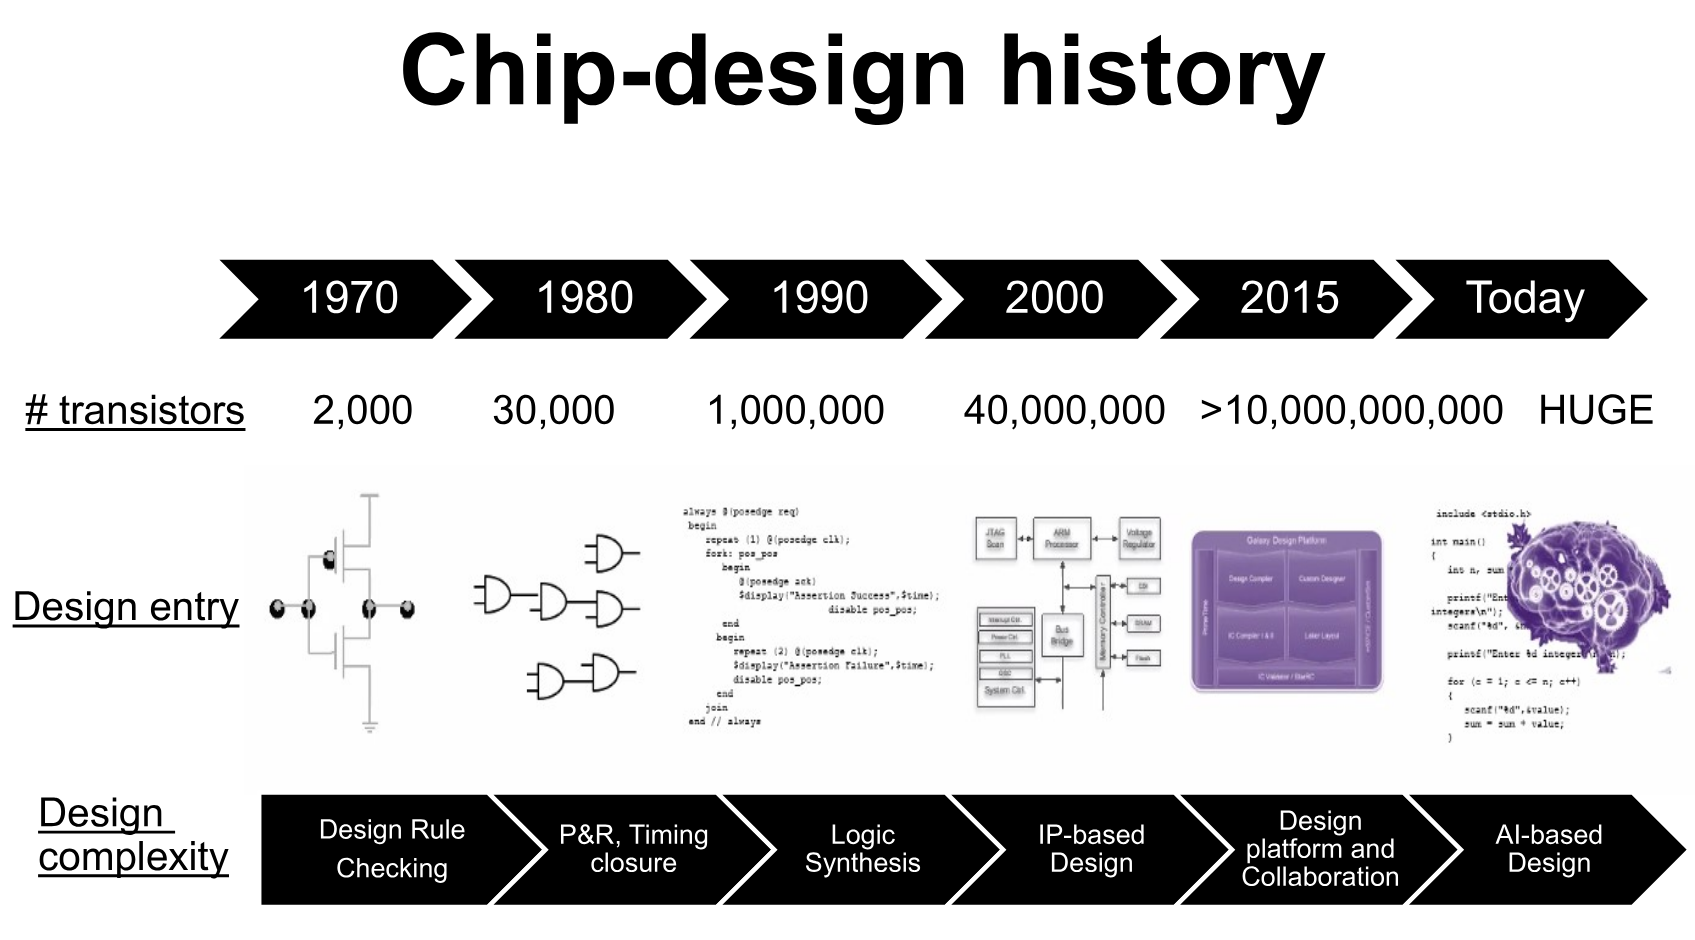
\includegraphics[scale=0.3]{../figures/chip_histo.png}
\end{center}

Many technologies are available to streamline chip design (for instance, \textit{synthesis} and automated tools).
Having more transistors within a single processor also allows for advanced features.
For instance, something like a \textit{floating point} processing unity executing alongside the main processor takes a large number of transistors to implement, which larger chip transistor densities allow.

\subsubsection{Costs}

\textbf{Costs} have to be taken into account.
There are 2 main types of costs:
\begin{itemize}
	\item \textbf{Design} costs: they are largely \textit{fixed}/non-recurring costs (\textbf{NRE}) and grow rapidly with chip complexity and process-node sophistication;
	\item \textbf{Manufacturing} costs: we note that manufacturing costs are dominated by the cost for building a new fab, which explodes when movind to advanced semiconductor nodes.

	We also note that when evaluating manufacturing costs, it is important not to forget the impact of yield, i.e., the percentage of products that pass the test phase.
The production process for every product undergoes an evolution which normally leads to an improvement in yield (also known as learning curve).
When yield increases, the cost decreases.
More than 50\% of manufacturing cost is due to validation and testing procedures!
\end{itemize}

\subsubsection{Processor performance evolution}

Processor \textbf{performance} can be measured by counting the number of operations executed or the time needed to execute them.
\begin{itemize}
	\item User point of view: performance $=$ response time (time between start and completion of an operation);
	\item System manager point of view: performance $=$ \textit{troughput} (total amount of work done in the time unit).
\end{itemize}

Processor performance evaluation is often performed by letting the computer to execute
applications and observing its behavior.
Unfortunately, the choice of the applications severely
affects the performance.
In the ideal case, one should use as workload the mix of
applications the user will run.
However, they are normally unknown, and largely
variable from one user to another.
Therefore, some \textbf{benchmarks} are selected to mimic real
cases.

Processor performance has steadily increased since the 1970s, where the first mainframe machines started being ranked based on performance.

\begin{itemize}
	\item From the 1970s to around the 1980s, yearly performance increases were of about 25\%;
	\item In the 1980s, the introduction of \textbf{RISC} (\textit{Reduced Instruction Set Computer}) architectures, as opposite to \textbf{CISC}, led to a yearly performance gain of around 50\%;
	\item In the first years of the 2000s, processor performance growth hit a slow down because aiming for higher and higher clock speeds became unfeasible (mainly because of power dissipation constraints). This was disadvantageous for the \textit{superscalar} architectures used at the time, characterized by high pipeline depth and instruction level parallelism;
	\item The solution most vendors adopted from the mid 2000s onwards, and which to this day is widely adopted, is \textit{multi-core} processors. In a \textit{multi-core} processor, we effectively have multiple processors (or processor \textit{cores}) running in parallel on a single, or multiple tasks. Note that multi-core setups increase \textit{throughput}, and not \textit{response time}.
\end{itemize}

Today, we can talk about the fact that modern computer systems employ various types of \textit{accelerators}, that is circuits intended to support specific applications alongside the CPU, like graphics or AI.

In the recent years, the widespread adoption of Artificial Intelligence (AI) applications prompted the introduction of new computing architectures denoted as AI accelerators, such as \textbf{GPU}s (\textit{Graphics Processing (Units)}).
GPUS were originally introduced for graphics applications, but their current success is due to their ability to effectively manage large and regular data structures.
The GPU market (in 2024 corresponding to about 18 B\$), is expected to grow to 406 B\$ by 2033 (with a Compound Average Grow Rate, or \textit{CAGR}, of 41,39\%). The CAGR of the CPU market is about 7\%.

\subsubsection{The computer market}

The computer \textit{market} is currently split in 5 different areas:
\begin{itemize}
	\item \textit{Personal Mobile Devices} (\textbf{PMD}s): this area includes smartphones and tablet computers. Emphasis is on energy efficiency and real-time applications. Here, system price is around \$100 - \$1,000, with the microprocessor price at \$10 - \$100.
		Architectures are usually highly parallel (and in fact smartphones were the earliest devices to make heavy use of multi-core processors); 
	\item Desktop computing: this area covers from PCs to workstations (and in some sense, even laptops). The main target of this area is to optimize the price-performance ratio. The system price is around \$300 - \$2,500, and of course the microprocessor price follows \$50 - \$500. Power is much less important than before, as we don't use batteries but power off the grid;
	\item Servers: these systems provide larger-scale and more reliable computing services.
		The main parameters of products in this area are:
		\begin{itemize}
\item Availability;
\item Scalability;
\item Throughput.
		\end{itemize}
System price is around \$5,000 - \$10,000,000, with microprocessor price around \$200 - \$2,000;
	\item Clusters / \textit{Warehouse Scale Computers} (\textbf{WSC}): systems that offer “Software as a Service (\textit{Saas})” or “Platform as a Service (\textit{PaaS})”.
The emphasis is on availability, price-performance, and power consumption.
\textit{Supercomputers} make up a part of this category, where the emphasis is on floating-point performance and fast internal networks.
The system price is high at around \$100,000 - \$200,000,000, with the microprocessor price around \$50 - \$250 (because at times we might use off the shelf processors in massively parallel setups);
	\item Embedded computers: this area is a major application area of the computer
market. It covers all special-purpose computer-based applications (from microwaves to coffee machines, from automotive to videogames).
Adopted microprocessors vary from cheap low-end 8-bit processors to very efficient (and expensive) high-end processors.
The system price ranges from \$10 - \$100,000, with microprocessor price at around \$0.01 - \$100 (possibly extremely cheap).

Special reguirements often existing in this area are:
\begin{itemize}
\item Real-time performance reduirements;
\item Memory minimization;
\item Power consumption minimization;
\item Reliability constraints.
\end{itemize}

 Embedded problems are often solved resorting to one of the following "standard" solutions:
\begin{itemize}
	\item Standard processor, custom logic, custom software. We call the combination of standard processors with custom logic \textbf{ASIC} (\textit{Application Specific Integrated Circuit});
	\item Standard processor, custom sofware;
	\item Standard DSP, custom software.
\end{itemize}

Programmable devices (such as \textbf{FPGA}s) are playing a growing
role.

\end{itemize}

\subsubsection{Power}

Continuous increase in system complexity and device integration often leads to problems with \textbf{power consumption.}
Power consumption may be critical under two aspects:
\begin{itemize}
	\item \textbf{Power}: \textit{static} power, consumed when a device is just running without doing work, and \textit{dynamic} power, which mainly depends on the frequency devices run at (and also the square power). i
	Until now it has been dominated by dynamic power, i.e., that consumed by each transistor when switching between different states.
The dynamic power for each transistor can be evaluated by the usual formula:
$$
P_{dynamic} = f V^2 C_{eq}
$$
whereas static power can be evaluated by:
$$
P_{static} = V I
$$
For this reason, voltage continuously dropped in the last years.

	\item \textbf{Energy}: it is given by:
$$
E = C_{eq} V^2 
$$
It is mainly of interest for mobile devices.
\end{itemize}

\subsubsection{Depedendability}

\textbf{Dependability} is the quality of the system to deliver a
correct service.
Dependability of computer systems is traditionally very
high, but it can be lowered by:
\begin{itemize}
\item Bugs in the design of the hardware;
\item Bugs in the software;
\item Defects in the hardware (introduced by the manufacturing process);
\item Faults happening during the product operation.
\end{itemize}

Many \textbf{safety critical} systems exist.
In the past, possible misbehaviors of computer systems were critical in some areas, such as
\begin{itemize}
\item Space;
\item Avionics;
\item Nuclear plants control.
\end{itemize}

In more recent years, computer-based systems
expanded to other safety-critical areas, such as:
\begin{itemize}
\item Rail-road traffic control
\item Automotive
\item Biomedical
\item Telecommunications.
\end{itemize}

Dependability \textit{metrics} exist.
Dependability is often measured using:
\begin{itemize}
	\item \textit{Mean Time To Failure} (\textbf{MTTF}) or \textit{Failures In Time} (\textbf{FIT}), which is the reciprocal. 1 FIT equals 1 failure in one billion hours;
	\item \textit{Mean Time To Repair} (\textbf{MTTR});
	\item \textit{Mean Time Between Failures} (\textbf{MTBF}).
\end{itemize}

The three measures are related by the formula:
$$
MTBF = MTTF + MTTR
$$
Finally, availability is the probability that a system works correctly in a generic time instant (usually measured in FITs).

We provide a figure of the typical \textit{bathub curve} that describes the probabilty of faults given the age of a component.
\begin{itemize}
	\item The \textit{infant mortality} zone is where faults of components show themselves early. Controlled \textit{burn-in} can partially solve this problem;
	\item The \textit{normal life} zone is where expect to spend time using devices;
	\item The \textit{end of life} zone is where failures hidden in components which otherwise worked fine start appearing. This is of particular interest to data centers where components are heavily stressed.
\end{itemize}

\begin{center}
	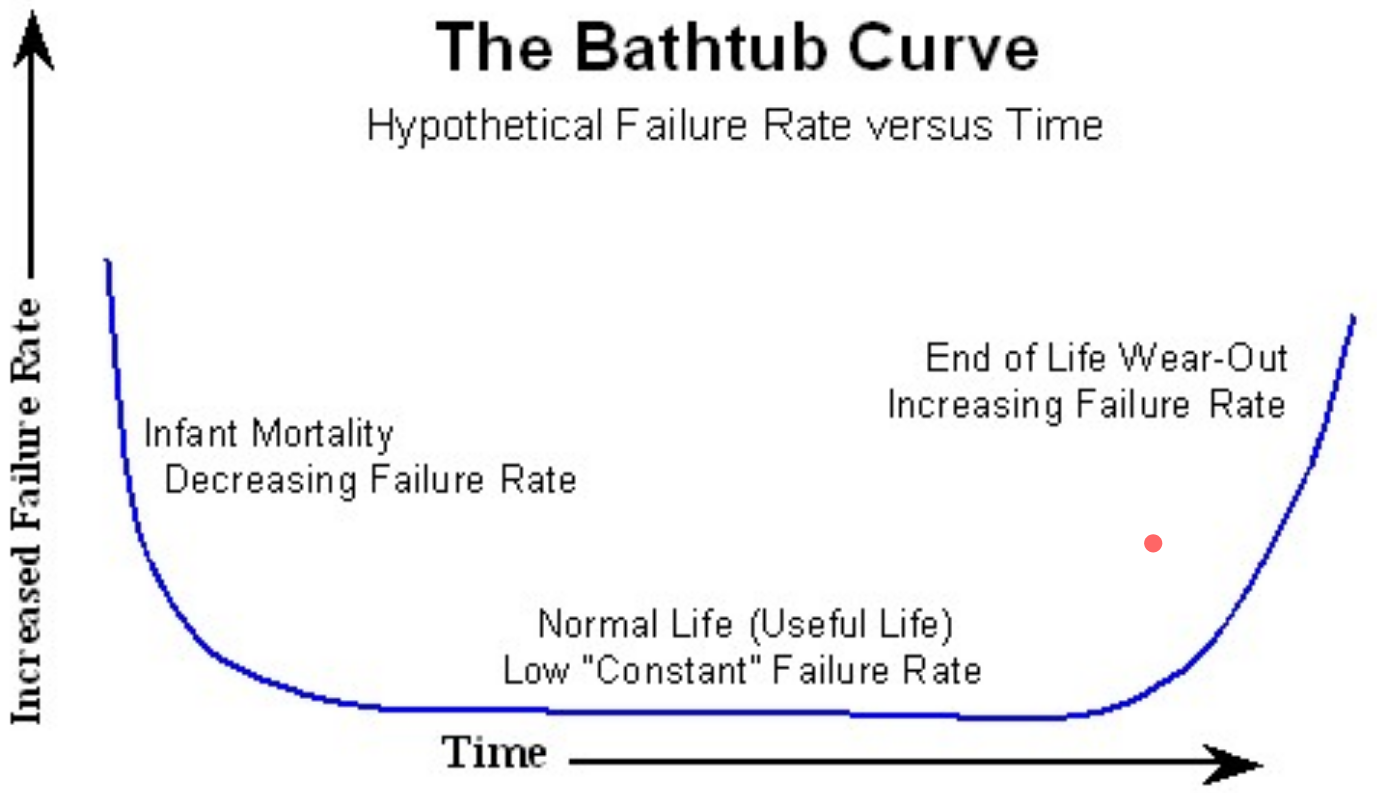
\includegraphics[scale=0.3]{../figures/bathub_curve.png}
\end{center}

\subsubsection{Reproducibility}
Going back to the topic of \textit{performance}, we introduce \textbf{reproducibility}.
Information about execution times on benchmarks
should allow reproducibility.
This means reporting detailed information about:
\begin{itemize}
\item Hardware (system configuration);
\item Software (OS, compiler, program);
\item Program input.
\end{itemize}

A common issue is comparing and summarizing
performance:
\begin{itemize}
\item \textbf{Problem 1}:
I know the performance of one machine on a set of
programs: which is its global performance?
\item \textbf{Problem 2}:
I know the performance of two machines on the same
set of programs: which is their relative performance?
\end{itemize}
A number of metrics have been proposed, such as total execution time, arithmetic mean and weighted means.

\subsubsection{Ahmdal's law}

\begin{definition}{Ahmdal's law}
We define the \textit{speedup} from a given architecture enhancement as:
$$
\text{speedup} = \frac{\text{performance with enhancement}}{\text{performance without enhancement}}
$$
\end{definition}

The speedup resulting from an enhancement depends on two factors:
\begin{itemize}
\item $\text{fraction}_\text{enhanced}$: the fraction of the computation time that takes advantage of the enhancement;
\item $\text{speedup}_\text{enhanced}$: the size of the enhancement on the parts it affects.
\end{itemize}

We can compute the execution time after the speedup as:
$$
\text{execution time}_\text{new} = \text{execution tiem}_\text{old} \cdot \left(  \right)
$$

Applying the definition of speedup, we get:
$$
\text{speedup} = \frac{\text{performance with enhancement}}{\text{performance without enhancement}} = \frac{1}{ (1 - \text{fraction}_\text{enhanced}) + \frac{\text{fraction}_\text{enhanced}}{\text{speedup}_\text{enhanced}} }
$$

Ahmdal's law is particularly useful in the study of parallel architectures, as it expresses the speedup given by optimizing parallelizable parts of computing tasks.
More specifically, we use it to explain why we can never have $S = N$ with $N$ processor cores. 

We can say that there will always be intervals of sequential execution ($T_\text{seq}$), spent executing instructions that cannot be parallelized, such as I/O operations, conditional statements, inherently sequential algorithms, etc...
Then the speedup $S$ can be defined as:
$$
S = \frac{T_1}{T_{\text{seq}} + \frac{T_1 - T_\text{seq}}{N} }
$$
with $T_1$ being the full execution time, i.e., the speed-up gain comes only from the parallelizable parts of the program ($T_1 - T_\text{seq}$), while the sequential parts ($T_\text{seq}$) cannot benefit significantly from parallelism.

The problem is that, taking the limit for $N \rightarrow \infty$, we obtain:

$$
\lim_{N \rightarrow \infty} S =
\lim_{N \rightarrow \infty}
\frac{T_1}{T_{\text{seq}} + \frac{T_1 - T_\text{seq}}{N}}
= \frac{T_1}{T_\text{seq}}
$$

Thus, as $N$ increases, the speed-up becomes dominated by the sequential parts: the parallelizable portions are progressively reduced, while the sequential portions remain and ultimately become the limiting factor for the overall system performance.

\subsubsection{The CPU performance equation}

Let's talk about measuring the time required to
execute a program
There are several possible approaches:
\begin{itemize}
\item By observing the real system;
\item By simulation;
\item By applying the \textbf{CPU performance equation}.
\end{itemize}

\begin{definition}{CPU performance equation}
CPU execution time is given by:
$$
\text{CPU Time} = \left( \sum_i \text{CPI}_i \times \text{IC}_i \right) \times T_C
$$
where:
\begin{itemize}
	\item $\text{CPI}_i$ is the number of clock cycles required by instruction $i$;
	\item $\text{IC}_i$ is the number of times instruction $i$ is executed in the program;
	\item $T_C$ is the clock period.
\end{itemize}
\end{definition}

This equation is quite basic, as it doesn't take any processor optimizations into account.
Still, it is a feasible metric for processor performance estimation, before the processor is even actually implemented.

\subsection{Instruction Set Principles}

Every processor owns an \textit{Instruction Set Architecture} (\textbf{ISA}).
The ISA provides the information about the processor reduired by programmers and
compilers to produce correctly working code:
\begin{itemize}
	\item The set of available \textit{instructions};
	\item Instruction \textit{encodings};
	\item Available \textit{registers};
	\item etc...
\end{itemize}

Different processors may share the same ISA (e.g., Intel and AMD processors, or processors of the same family).

The Instruction Set Architecture (ISA) is basically how the computer
is seen by the programmer or the compiler.
There are many alternatives possible for the ISA designer,
any choice modifies the way to encode the instructions.
The different alternatives may be evaluated in terms of:
\begin{itemize}
\item Processor performance;
\item Processor complexity;
\item Compiler complexity;
\item Code size;
\item Power consumption;
\item etc...
\end{itemize}
Different product areas may assign different weights to the
above parameters.

An ISA specification is particulary important because it is usually the only set of information released by a company about a processor.
Of course, the internal implementation details are trade secrets, but the ISA specification is made available in order to allow programmers to develop for a certain platform.

\subsubsection{CPU taxonomies}

CPUs (and their ISAs) are often classified according to the type of their internal storage:
\begin{itemize}
\item Stack;
\item Accumulator;
\item Registers:
	\begin{itemize}
	\item Register-memory, as in x86;
	\item Register-register (load-store). Basically all RISC architectures are of this kind;
	\item Memory-memory (no real cases).
	\end{itemize}
\end{itemize}

\begin{center}
	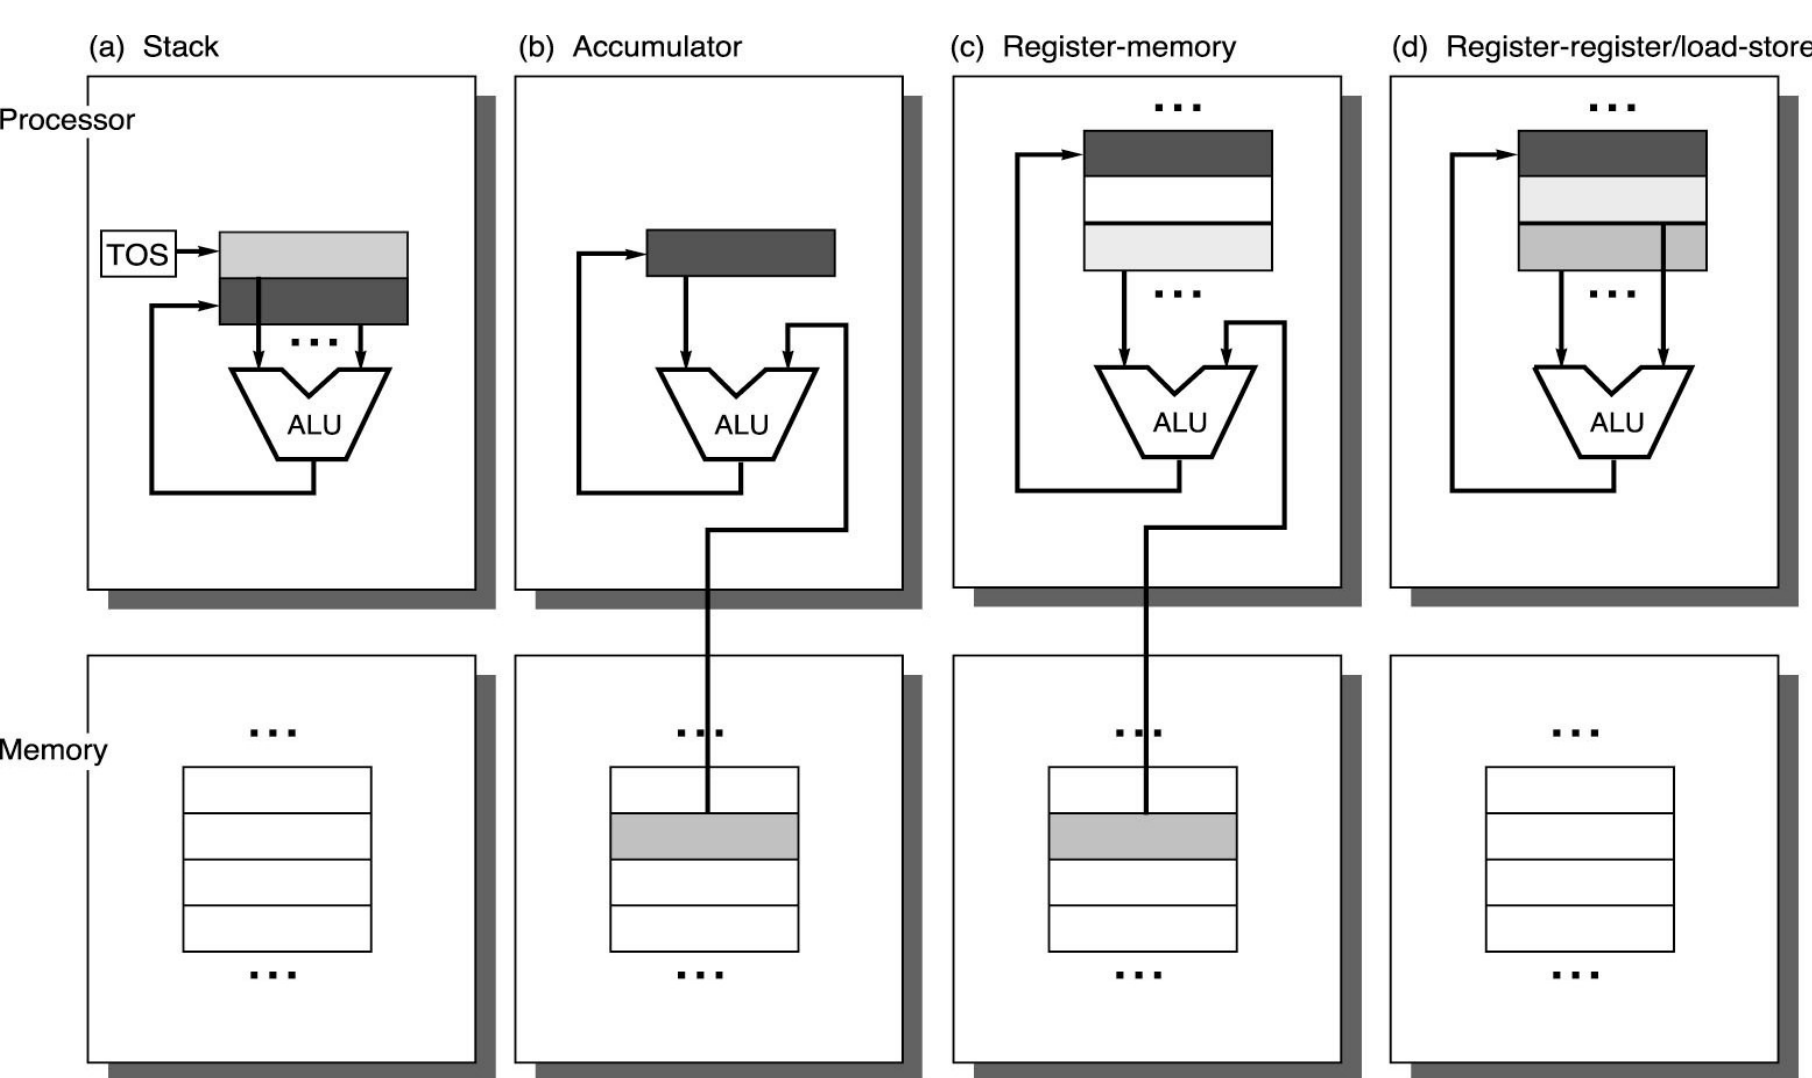
\includegraphics[scale=0.3]{../figures/taxonomies.png}
\end{center}

Currently, all processors are \textit{General-Purpose Register} (\textbf{GPR}) machines.
The reason for this is:
\begin{itemize}
\item Registers are faster than memory;
\item Registers are easier for a compiler to use (or better, to \textit{optimize}).
\end{itemize}

CPUs can also be classified according to:
\begin{itemize}
\item Typical number of operands per ALU instruction (2 or 3). In RISC-V and ARM, this is almost always 2;
\item Typical number of memory operands per ALU instruction (from 1 to 3, for architectures that feature memory operands in the first place in instructions rather than load/store).
\end{itemize}

\subsubsection{Memory addressing}

We have some orthogonal characteristics relating to memory \textit{addressing}:
\begin{itemize}
	\item \textbf{Little Endian} vs. \textbf{Big Endian}: processors usually address memory in bytes, organized into words. The order of the bytes within a word matters:
	\begin{itemize}
		\item \textit{Little Endian} puts the byte with the lowest address (X...X000) at the least significant position. The address of the data is that of the least significant byte;
		\item \textit{Big Endian} puts the byte with the lowest address (X...X000) at the most significant position. The address of the data is that of the most significant byte.
	\end{itemize}
\item \textbf{Aligned} vs. \textbf{misaligned} accesses:
	\begin{itemize}
		\item \textit{Aligned} means allowing only aligned accesses not straddling word (usually 2 byte) bounds. It is a limitation;
		\item \textit{Disaligned} access, on the other hand, requires: hardware overhead and performance overhead.
	\end{itemize}
\end{itemize}

We shall also note that in GPR machines an addressing mode specifies a constant, a register, or a memory location (through its effective address).

We remember the addressing modes noted in section 1.2.5 for x86. Some of these are shared with ARM and RISC-V RISC architectures (mainly register mode, with destination register, immediate and displacement modes for load/store operations).

By carefully choosing the addressing modes, one can
obtain some important consequences:
\begin{itemize}
\item  Reducing the number of instructions;
\item  Increasing the CPU architecture complexity;
\item  Increasing the average \textit{Cycles Per Instruction} (\textbf{CPI}).
\end{itemize}

An interesting thing to note is the size devoted to immediate operands in immediate instructions.
That is, how large can the immediate value be, when it is embedded in the addressing part of the instruction?
Note that memory displacements basically are a special case of immediate operands, and as such fall in the same category and have the same problem.
In fact, we had already noted this issue in section 1.2.5.

An experimental evaluation can be performed.
\begin{center}
	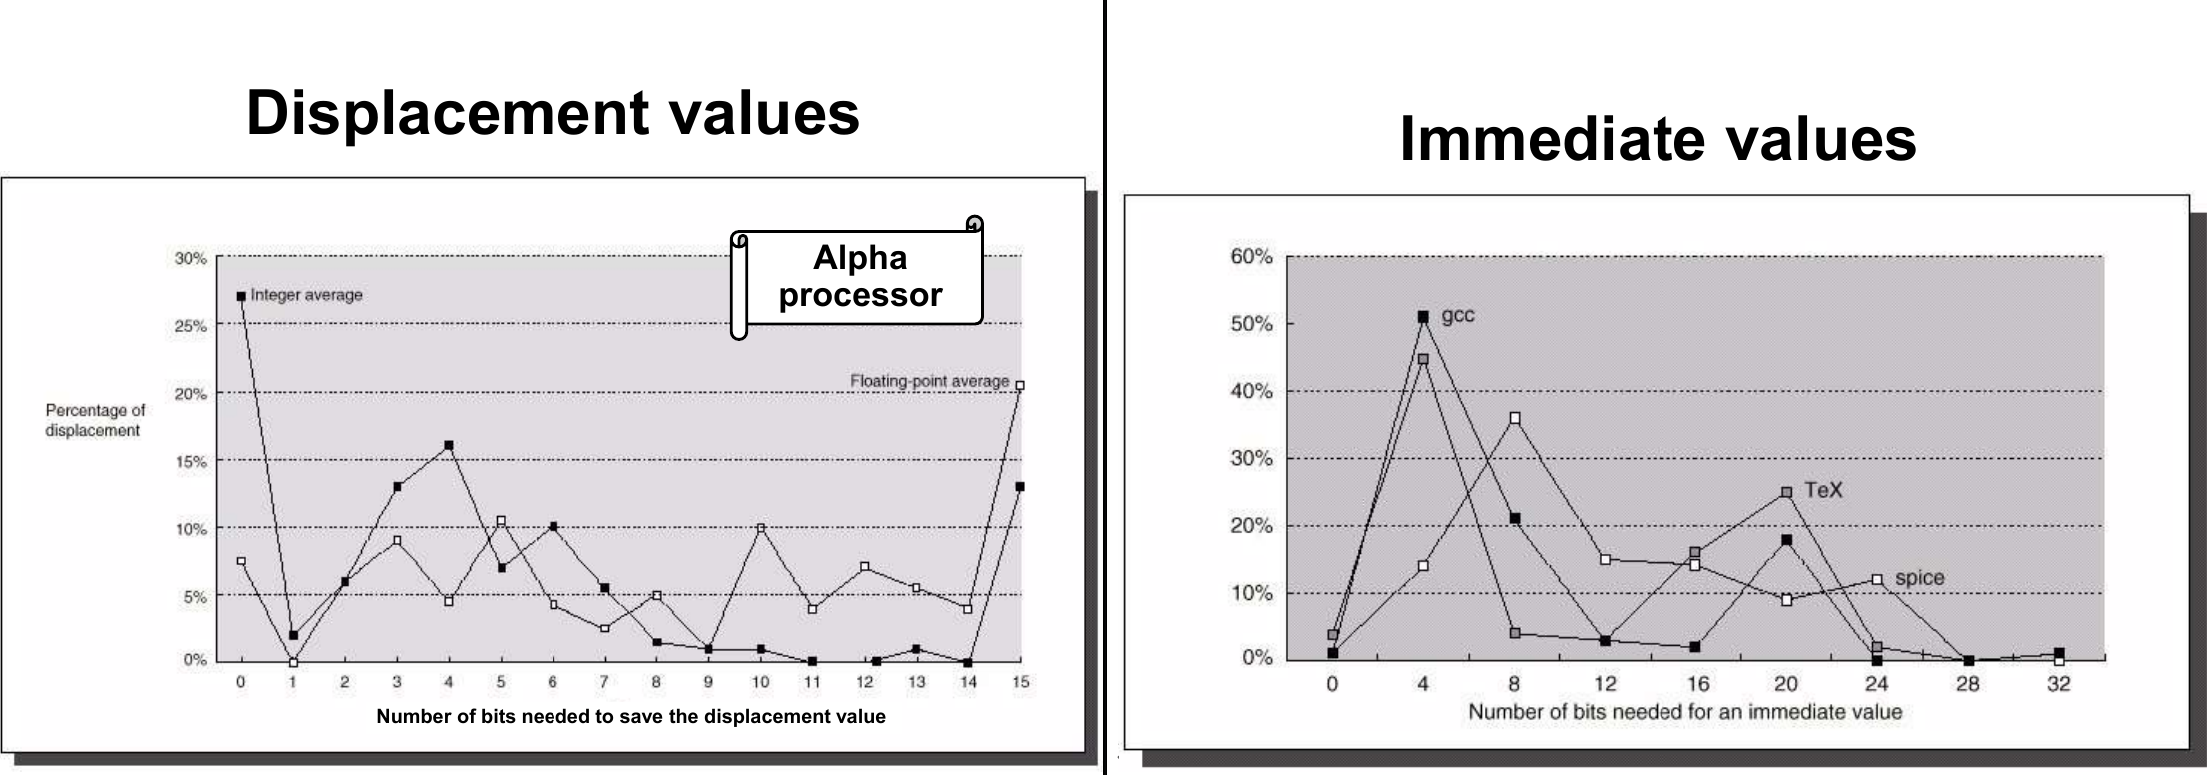
\includegraphics[scale=0.25]{../figures/disp_imm.png}
\end{center}

From the plots, compiled from a DEC alpha processor for displacement and for typical compiled applications for immediates, we get that:
\begin{itemize}
\item Displacement, immediate and register indirect modes represent from 75\% to 99\% of the addressing modes;
\item The address size for displacement mode should be from 12 to 16 bits (75\% to 99\% of the displacements);
\item The size of the immediate field should be at least 8 or 16 bits (50\% and 80\% of the cases, respectively).
\end{itemize}

RISC-V uses the solution of doing 12 bits immediates.
As we previously stated, bigger immediates have to be transferred to register in multiple instructions.
This tradeoff is made valid by the simplicity gains of the processor architecture.

\subsection{Operations in the instruction set}

Clearly, a key component of an ISA is the \textbf{instruction set} made available to the programmer. 
Different categories of instructions exist:

\begin{table}[H]
	\center \rowcolors{2}{white}{black!10}
	\begin{tabular}{c | p{10cm}}
\hline
\textbf{Operator type} & \textbf{Examples} \\
\hline
Arithmetic and logical & Integer arithmetic and logical operations: add, and, subtract, or \\
\hline
Data transfer & Loads-stores (move instructions on machines with memory addressing) \\
\hline
Control & Branch, jump, procedure call and return, traps \\
\hline
System & Operating system call, virtual memory management instructions \\
\hline
Floating point & Floating-point operations: add, multiply \\
\hline
Decimal & Decimal add, decimal multiply, decimal-to-character conversions \\
\hline
String & String move, string compare, string search \\
\hline
Graphics & Pixel operations, compression/decompression operations \\
\hline
\end{tabular}
\end{table}

We should be making the common case fast: not all the instructions are executed with the same frequency!
When designing and implementing an instruction set, the most commonly executed instructions should be made faster than others.

\end{document}
